%!TEX root = ../../thesis.tex

\section{HTTP Range Requests and Cloud Optimisation}
\label{methodology:http_range_requests}

A critical component of cloud-optimised geospatial formats is their ability to support selective data retrieval without downloading entire datasets. FlatCityBuf achieves this capability through strategic implementation of HTTP Range Requests \citep{http_range_requests}, enabling efficient partial data retrieval. This section details the technical implementation, optimisation strategies, and cross-platform compatibility of this mechanism.

\subsection{Principles of Partial Data Retrieval}
\label{methodology:http_range_requests:partial_retrieval_principles}

HTTP Range Requests, defined in RFC 7233 \citep{rfc_7233}, allow clients to request specific byte ranges from server resources instead of entire files. This capability is fundamental to FlatCityBuf's cloud-optimised design. Since each feature in FlatCityBuf is length-prefixed, once the client knows the byte offset to a specific feature, it can request precisely the bytes needed. While data access patterns vary—from sequential access to spatially or attribute-indexed retrieval—the core principle remains consistent: fetch only the necessary data.

\subsection{Range Request Workflow}
\label{methodology:http_range_requests:range_request_workflow}

The HTTP Range Request workflow in FlatCityBuf follows a carefully optimised sequential process:

\begin{enumerate}
  \item \textbf{Header Retrieval}: The client first requests the magic bytes (8 bytes) and \texttt{Header} (described in \autoref{methodology:header:schema_indexing}). This initial request provides essential metadata including coordinate reference systems, transformations, the total number of features, and index structure information \etc.

  \item \textbf{Index Navigation}: Based on query parameters (spatial bounding box or attribute conditions), the client selectively navigates the appropriate index structures:
    \begin{itemize}
      \item For spatial queries, the client traverses only the relevant nodes of the packed Hilbert R-tree along the query path
      \item For attribute queries, the client similarly traverses only the necessary portions of the appropriate \ac{s+tree} indices
    \end{itemize}

  \item \textbf{Feature Resolution}: Using byte offsets obtained from the indices, the client makes targeted range requests for specific features. The size of each feature is determined implicitly by the difference between consecutive offsets. The absolute byte offset of a feature within the file can be calculated by summing the size of the \texttt{Magic bytes}, the size of the \texttt{Header}, the size of the \texttt{indices}, and the relative offset of the feature.

  \item \textbf{Progressive Processing}: Features are processed incrementally as they arrive, allowing applications to begin rendering or analysis before all data is received, significantly improving perceived performance.
\end{enumerate}

This workflow enables efficient partial data retrieval by leveraging indexing strategies to minimize both the number of HTTP requests and the total data volume transferred.

\begin{figure}[htbp]
  \centering
  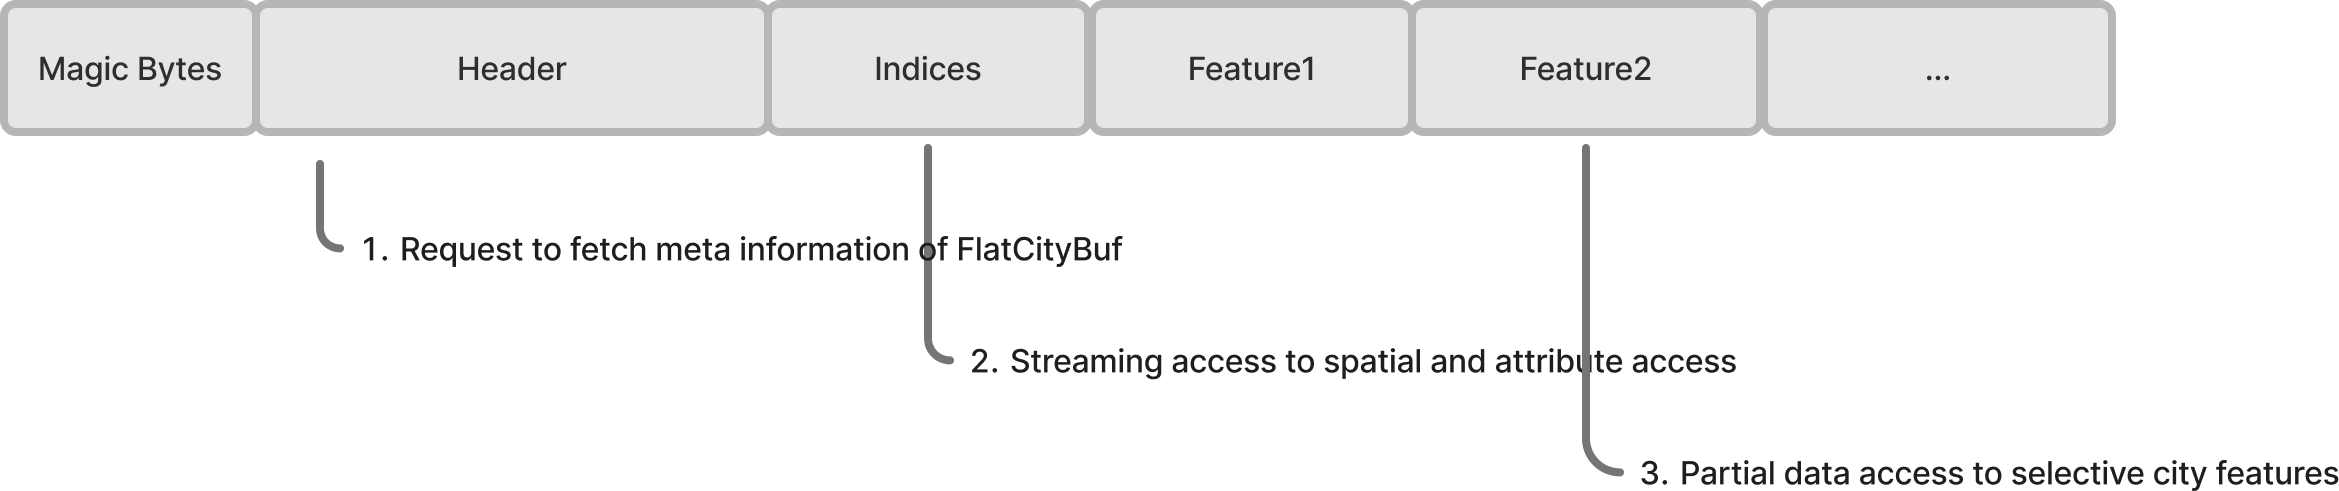
\includegraphics[width=0.9\textwidth]{figs/methodology/range_request_workflow.png}
  \caption{HTTP Range Request workflow in FlatCityBuf showing the sequential process of header retrieval, index navigation, and selective feature retrieval. The client makes targeted requests for specific byte ranges rather than downloading the entire dataset.}
  \label{fig:methodology:http_range_requests:range_request_workflow}
\end{figure}

\subsection{Optimisation Techniques}
\label{methodology:http_range_requests:range_request_optimisations}

Network latency often dominates performance when accessing data over HTTP, with each request incurring significant overhead regardless of payload size. FlatCityBuf implements several techniques to minimise this overhead:

\begin{itemize}
  \item \textbf{Request Batching}: Multiple feature requests are grouped into larger, consolidated HTTP requests rather than making individual requests for each feature. This approach significantly reduces the number of HTTP round trips, improving overall performance while minimizing network overhead.

  \item \textbf{Payload Prefetching}: When an attribute index is about to be used, the implementation proactively downloads a portion of its payload section. This anticipatory approach reduces latency for subsequent operations by having relevant data already available in memory when needed.

  \item \textbf{Streaming Process of Indices}: Both spatial and attribute indices implement a streaming approach where only the necessary node items in the tree structure are loaded when needed. Rather than loading entire index structures upfront, the system traverses the tree on demand, requesting only the relevant portions required for the current query.

  \item \textbf{Buffered HTTP Client}: The implementation uses a buffered HTTP client that caches previously fetched data ranges, avoiding redundant requests when overlapping ranges are accessed.

\end{itemize}

These optimisations work in concert to minimise the number of HTTP requests, resulting in significantly improved performance for cloud-based 3D city model applications.

\subsection{Cross-Platform Implementation}
\label{methodology:http_range_requests:cross_platform_implementation}

FlatCityBuf provides range request capabilities across multiple platforms to maximise accessibility and integration options:
\subsubsection{Cross-Platform Support}
\label{methodology:http_range_requests:cross_platform_implementation:cross_platform}

FlatCityBuf is implemented primarily as a Rust library that can be used in both native environments and web browsers. The same codebase is compiled to:

\begin{itemize}
  \item Native Rust library for server-side applications and desktop GIS tools
  \item WebAssembly (WASM) module for browser-based applications with JavaScript interoperability
\end{itemize}

This cross-platform approach enables FlatCityBuf to work with both Rust's native HTTP clients and browser-based Fetch API implementations. The WASM implementation has one notable limitation: current browser WebAssembly implementations use a 32-bit memory model (4GB limit), which may constrain processing of country-level datasets. This limitation will be resolved with the upcoming WebAssembly Memory64 proposal \citep{WebAssemblyCoreSpecification2}.

\subsection{Integration with Cloud Infrastructure}
\label{methodology:http_range_requests:cloud_integration}

The HTTP Range Request mechanism integrates seamlessly with modern cloud infrastructure. FlatCityBuf files can be served from standard object storage services like AWS S3, Google Cloud Storage, or Azure Blob Storage, all of which support range requests without additional server-side processing. This enables a serverless architecture where the client-side filtering approach eliminates the need for dedicated server-side processing. This infrastructure compatibility ensures that FlatCityBuf can be deployed in cost-effective cloud environments without requiring specialised application servers and databases.

\begin{figure}[htbp]
  \centering
  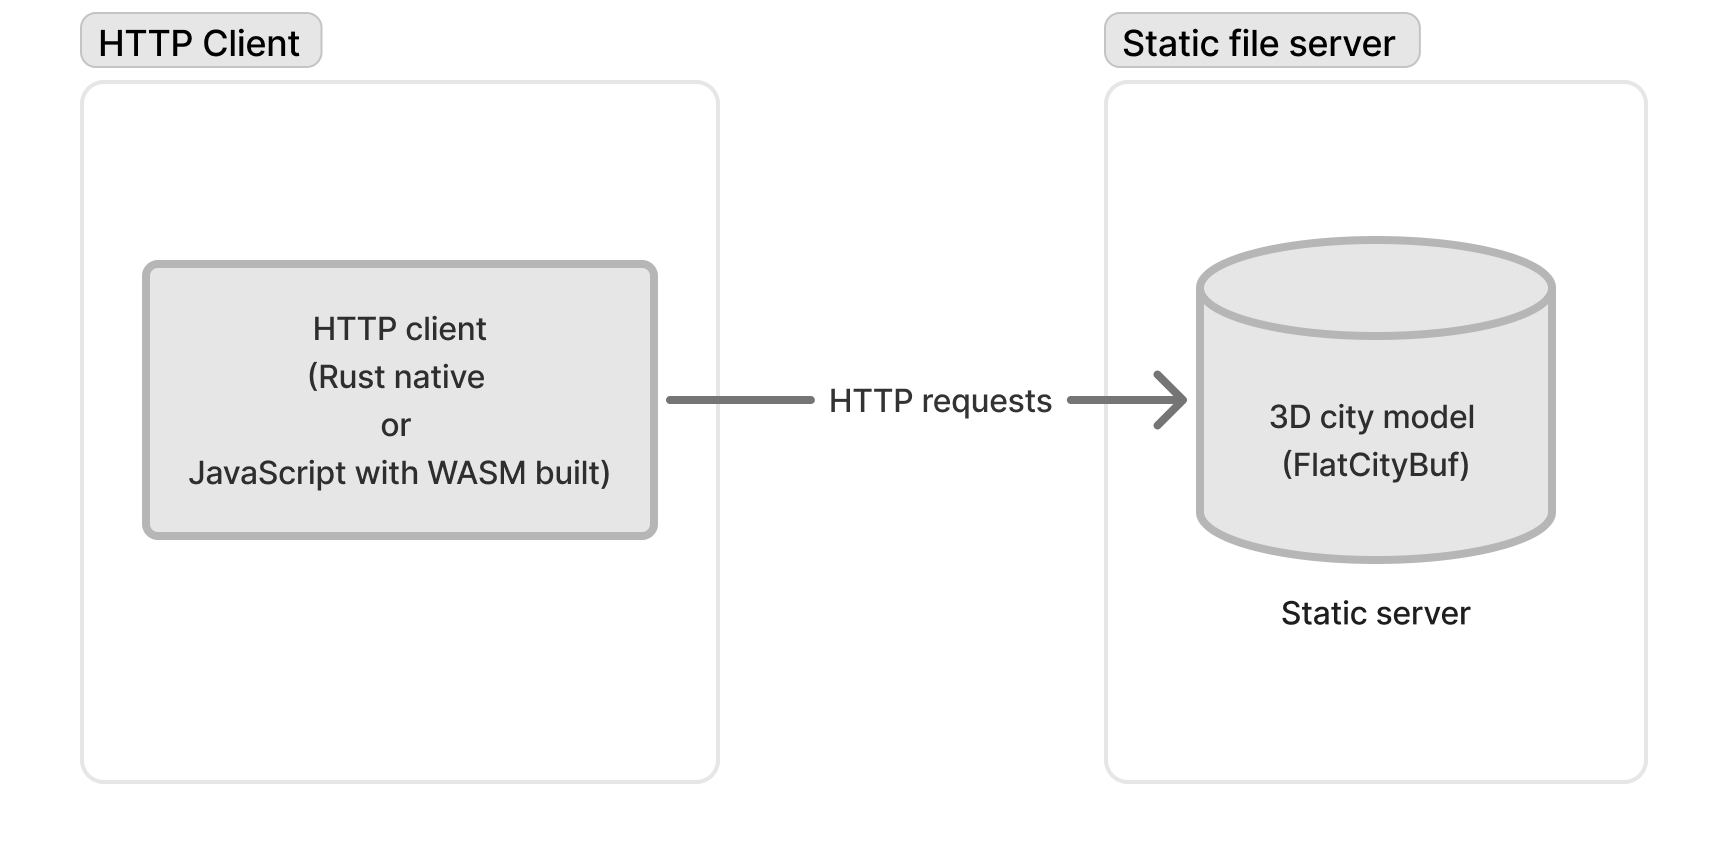
\includegraphics[width=0.9\textwidth]{figs/methodology/server_architecture_fcb.png}
  \caption{Server architecture for FlatCityBuf. The client-side filtering approach eliminates the need for dedicated server-side processing.}
  \label{fig:methodology:http_range_requests:server_architecture}
\end{figure}
